% E8 (SCRUM-59): Appendices: Figures 1 and 1b updated to the core scope, the model table, the
% assumptions table (from E4), E5's formulas and the data sources with download dates
% (lepton-plan.md, E8).
% E8 sets their order; \appendix numbers their tables A1, B1, ... (lepton.sty).
% Figures A1 and A2 are the Methodology document's (9 October 2026) Figure 1 and its next
% diagram, the Layer 1 pipeline, redrawn as built by src/diagrams.py (python -m src.diagrams,
% copied from results/e8_fig_*.png). The model table follows config.py, src/baselines.py,
% src/m3.py, src/m4.py and src/forecast_range.py; the data sources table, the notes in data/raw/.
\clearpage
\onecolumn
\appendix

\section{Study Design}\label{app:design}

\begin{figure}[h]
\centering
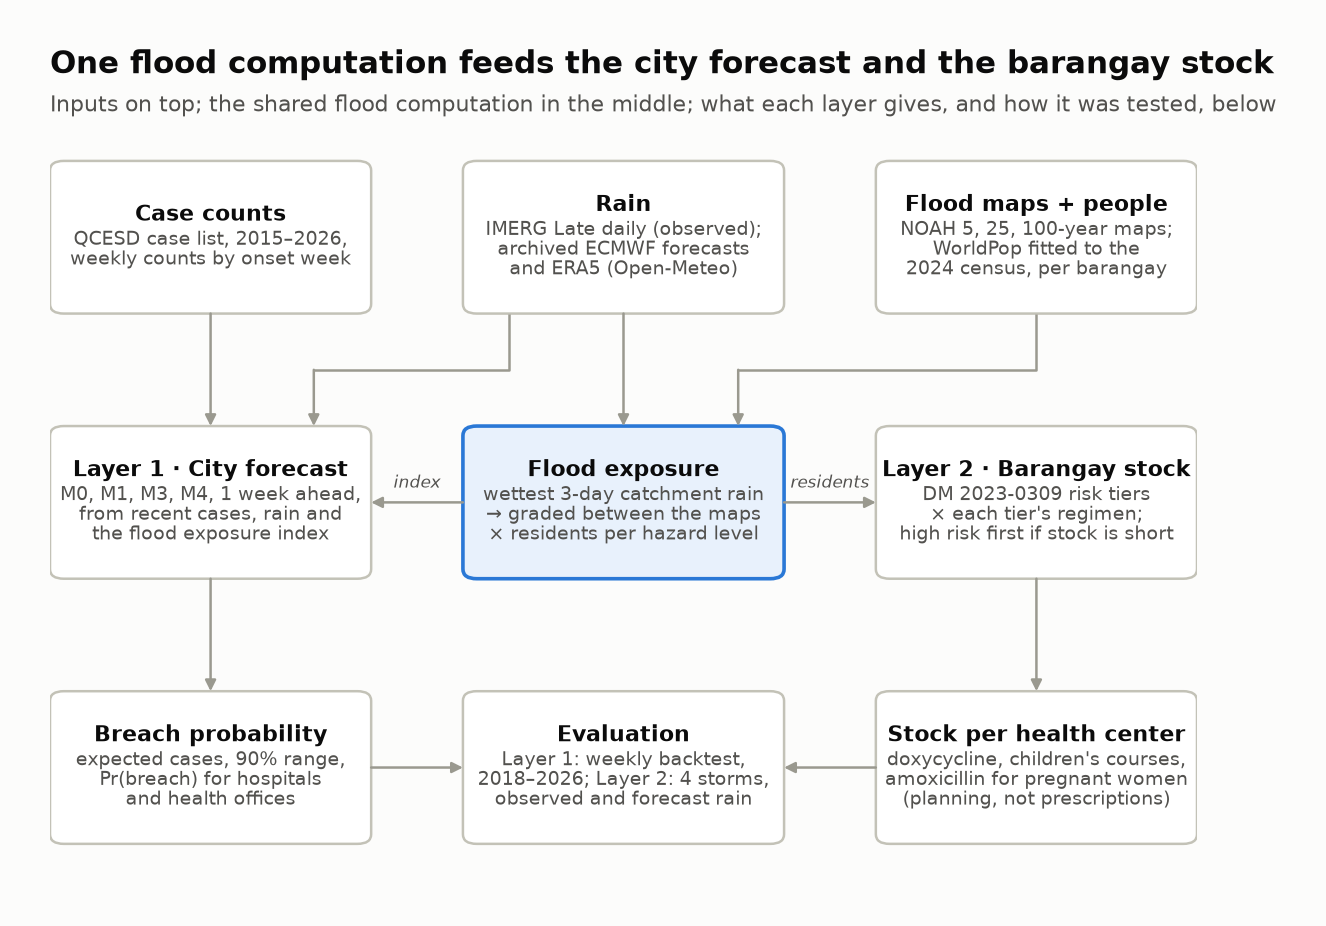
\includegraphics[width=0.94\textwidth]{figures/e8_fig_design.png}
\caption{The study design, updated from the project's methodology to what was built: QC only,
weekly counts by week of onset, four models forecasting one week ahead, rain measured over three
days, and Layer~2 checked on four storms. The flood computation (blue) turns rain into exposed
residents for Layer~2 and into the flood exposure index for Layer~1. Stock figures are for
planning, not prescriptions.}\label{fig:design}
\end{figure}

\begin{figure}[h]
\centering
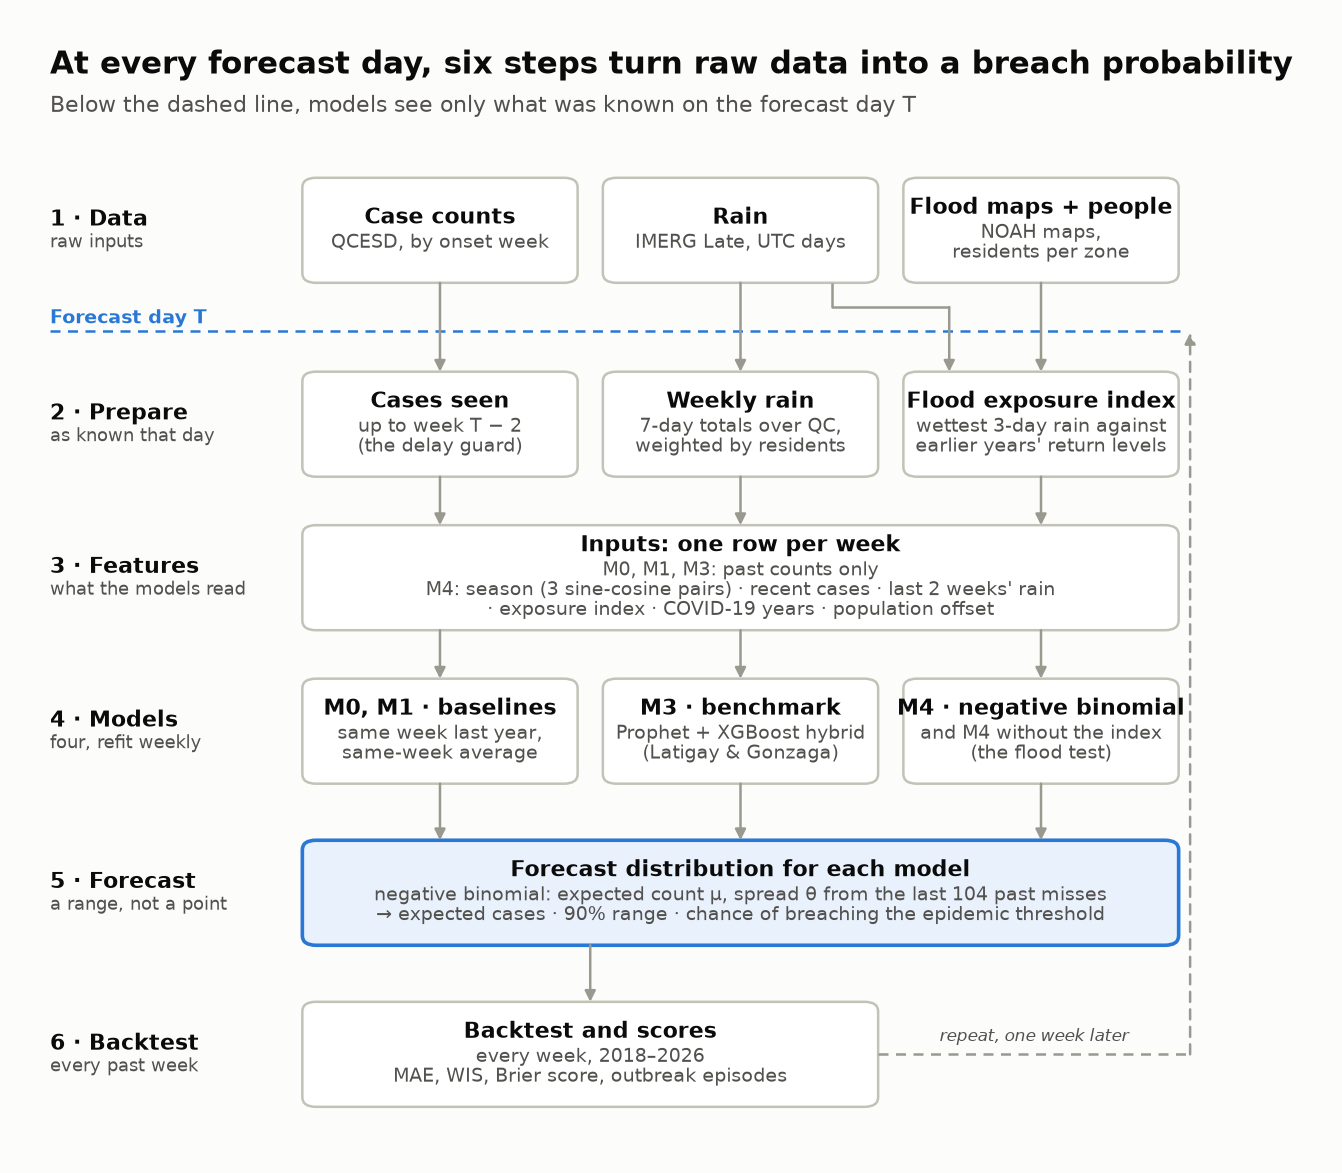
\includegraphics[width=0.94\textwidth]{figures/e8_fig_layer1.png}
\caption{Layer~1's steps at every forecast day. Rain and the flood exposure index are known on the
forecast day; case counts only up to two weeks before it (the delay guard). The backtest repeats
the six steps once a week, refitting every model each time.}\label{fig:layer1}
\end{figure}

\clearpage
\section{Models}\label{app:models}

{\footnotesize
\renewcommand{\arraystretch}{1.25}
\begin{longtable}{@{}>{\raggedright\arraybackslash}p{0.13\textwidth}
                    >{\raggedright\arraybackslash}p{0.26\textwidth}
                    >{\raggedright\arraybackslash}p{0.29\textwidth}
                    >{\raggedright\arraybackslash}p{0.24\textwidth}@{}}
\caption{The four models of Layer~1 and the flood test's variant. Each forecasts the count of the
week after the forecast day from what the delay guard lets it see, and is refitted at every
forecast day. The formulas are in Table~\ref{tab:formulas}; the file that computes each model is
named in small type.}\label{tab:models}\\
\toprule
\textbf{Model} & \textbf{Forecast} & \textbf{Inputs and fit} & \textbf{Role} \\
\midrule
\endfirsthead
\multicolumn{4}{@{}l}{\textit{Table~\thetable, continued}}\\
\toprule
\textbf{Model} & \textbf{Forecast} & \textbf{Inputs and fit} & \textbf{Role} \\
\midrule
\endhead
\midrule
\multicolumn{4}{@{}r}{\textit{Continued on the next page}}\\
\endfoot
\bottomrule
\endlastfoot
M0, last year \cfg{baselines.py}
  & The count of the same week 52 weeks earlier
  & Past counts only; nothing is fitted
  & Baseline: what a health office knows without a model \\
M1, seasonal average \cfg{baselines.py}
  & The mean count of the same week of the year over the epidemic threshold's reference years
    (up to the five most recent complete years before the target year, at least three, without
    2020--2021)
  & Past counts only; nothing is fitted
  & Baseline, and the practical test: M4 must beat the usual week \\
M3, Prophet--XGBoost \cfg{m3.py, m3_port.py}
  & Prophet's forecast plus XGBoost's correction of it, floored at zero
  & Past counts. Prophet: multiplicative seasonality, changepoint prior scale 0.55, weekly and
    yearly seasonality, no holidays. XGBoost: Prophet's in-sample errors from Prophet's forecast
    and the ISO week; xgboost's defaults, 100 rounds
  & Benchmark \parencite{latigay2026}, rebuilt on its own national data before the port to QC;
    D5's primary endpoint compares M4 with it \\
M4, negative binomial \cfg{m4.py}
  & The expected count $\mu$ of a negative binomial regression with QC's population as an offset
  & Season (three yearly sine--cosine pairs), recent cases (the two newest counts it may see),
    the last two weeks' rain over QC, the flood exposure index (larger of the last two weeks'),
    the COVID-19 years. Maximum likelihood with statsmodels' \texttt{negativebinomial}, which
    estimates the overdispersion; a term constant in every training row is left out
  & The proposed model \\
M4 without the index \cfg{m4.py}
  & As M4
  & M4's inputs without the flood exposure index, on the same rows
  & The flood test: does the index help? \\
\midrule
Every model \cfg{forecast_range.py}
  & A negative binomial with mean $\mu$ and spread $\theta$: expected cases, 90\% range and
    Pr(breach)
  & $\theta$ from the model's last 104 forecasts outside 2020--2021 whose counts it may see;
    with fewer than 26, its training fit's (M4: $1/\alpha$; M3: Prophet's); Poisson when misses
    are no wider than Poisson's
  & Makes every model's ranges and breach probabilities comparable \\
\end{longtable}
}

\clearpage
\section{Assumptions}\label{app:assumptions}
% E4 (SCRUM-25): the assumptions table, which E4's limitations point to; E8 places it among the
% appendices. Rows = the 29 assumptions in lepton-plan.md ("Assumptions to state in the paper"),
% less option A's reported-share cut-off (not used: A13 chose option C), plus the choices the
% build added (Notes.md sections 1-2 and config.py). Each value is the one in config.py; the
% config.py name sits under each assumption. Task codes are in the comment at each row's end.
% A test marked \checkme has not been run yet: run it, or change the cell to "Stated".
{\footnotesize
\renewcommand{\arraystretch}{1.18}
\begin{longtable}{@{}>{\raggedright\arraybackslash}p{0.22\textwidth}
                    >{\raggedright\arraybackslash}p{0.43\textwidth}
                    >{\raggedright\arraybackslash}p{0.29\textwidth}@{}}
\caption{Every assumption in LEPTON, its value and how it was tested. Values are set once, in
the code's \texttt{config.py}, under the names shown in small type.}\label{tab:assumptions}\\
\toprule
\textbf{Assumption} & \textbf{Value} & \textbf{Tested or stated} \\
\midrule
\endfirsthead
\multicolumn{3}{@{}l}{\textit{Table~\thetable, continued}}\\
\toprule
\textbf{Assumption} & \textbf{Value} & \textbf{Tested or stated} \\
\midrule
\endhead
\midrule
\multicolumn{3}{@{}r}{\textit{Continued on the next page}}\\
\endfoot
\bottomrule
\endlastfoot
%
\multicolumn{3}{@{}l}{\textbf{\color{leptonnavy}Cases and the city forecast (Layer 1)}}\\
A case's week \cfg{QCESD_ONSET}
  & The MMWR week of its date of onset; the list's own morbidity-week column is not used
  & Stated: that column changes meaning between years \\ % A13
Delay guard \cfg{DELAY_GUARD_G}
  & 2 weeks: forecasting week $T+1$ at week $T$, every model sees counts up to week $T-2$
  & Rerun with 1 and 3 weeks: the same three verdicts (Table~\ref{tab:robustness}) \\ % B2, B6, D3, D4
When a week's count is final \cfg{CASES_COMPLETE_DAYS}
  & 17 days after the week ends; later weeks are missing, not zero
  & 99\% of cases were admitted within 17 days of onset; a lower bound, since the delay from
    admission to report is unknown \\ % A13
Repeated rows in the case list
  & The 136 rows that repeat another row are kept as separate cases
  & With them the list matches QCESD's published 2025 totals to within 1\% \\ % A13, S4
Epidemic threshold \cfg{THRESHOLD_SD}
  & The week's mean plus 2 standard deviations over the up to 5 most recent complete non-COVID
    years before the target year, at least 3
  & Stated; QCESD's own method is not known \\ % B7
Week 53 \cfg{MAX_WEEK}
  & Treated as week 52; a reference year's own week 53 is not used
  & Stated \\ % A3, B7, B8
COVID-19 years \cfg{COVID_YEARS}
  & 2020--2021: an indicator in M4; not threshold reference years; out of headline scores
  & Every score also computed over all years, as a check (Section~\ref{sec:results-checks})
    \\ % B5, B7, D
Forecast spread before 26 past forecasts \cfg{THETA_MIN_FORECASTS}
  & Each model's training fit: M4's fitted $\theta$; M0's and M1's own fits on the weeks they
    see; Prophet's in-sample fit for M3
  & Stated; used for about the first half of 2018 only \\ % B6, B9, B10
M3's XGBoost settings \cfg{M3_XGB_PARAMS}
  & xgboost's defaults with 100 rounds; the paper gives none
  & Rerun with a maximum depth of 2: hybrid error 26.04 on the paper's data \\ % B3, B9
M3's gap filling \cfg{M3_LOCKDOWNS}
  & Our reading of the paper's three steps: lockdown weeks are those under ECQ or MECQ
    (15 March--31 May and 4--18 August 2020), and the series has no row for ISO 2020 week 53
  & Our seasonal naive forecast then matches all eight of the paper's published scores for it
    \\ % B3
\midrule
\multicolumn{3}{@{}l}{\textbf{\color{leptonnavy}Rain and flood exposure}}\\
Trigger rain \cfg{RAIN_ACCUM_DAYS}
  & The wettest three consecutive UTC days of daily IMERG Late rain
  & The single wettest day, run as a comparison \\ % A4, C3
A storm's rain
  & Its wettest three-day total ending during the flood
  & Stated \\ % C8, C9 (Notes.md 2.2)
Rain area \cfg{CATCHMENT_OUTLETS}
  & HydroBASINS level-12 sub-basins draining to the Marikina, San Juan and Tullahan rivers, each
    rain cell weighted by its area inside them
  & Stated \\ % A7, C3
IMERG's first year \cfg{IMERG_KEEP_2000}
  & June--December 2000 kept
  & Refit without it: return levels move by under 1~mm, the exposure index by at most 0.1
    point \\ % C3
Return-level fit \cfg{GUMBEL_MIN_YEARS}
  & Gumbel, on the annual maxima of at least 10 years before the forecast or storm year,
    refitted each year
  & Stated \checkme{the plan's one GEV refit for Carina was not run} \\ % C3
No-flood floor $R_0$ \cfg{R0_FACTOR}
  & $R_0 = 0.5\,\hat{R}(5)$, fixed
  & Stated; tuning it is future work \\ % C3
ERA5 fit years \cfg{ERA5_YEARS}
  & June 2000 to the year before each storm, the same years as IMERG
  & Stated \\ % A14, C9
Forecast model and lead times \cfg{FORECAST_LEADS_DAYS}
  & ECMWF IFS 0.25\textdegree, issued 1, 2 and 3 days before the rain
  & All four storms are in the archive \\ % A15, C9
Overlay rule
  & A pixel's residents count in proportion to its area inside a zone
  & Stated \\ % C2
Population map
  & WorldPop 2024, constrained 100~m (R2025A), fitted to each barangay's 2024 census total
  & Stated; Meta's map is future work \\ % A6, C1
Flood maps \cfg{NOAH_RETURN_PERIODS}
  & NOAH's 5-, 25- and 100-year Metro Manila maps, as published
  & The 11 barangays where a rarer map floods fewer residents were listed and inspected \\ % A8, C2
\midrule
\multicolumn{3}{@{}l}{\textbf{\color{leptonnavy}People and prophylaxis stock (Layer 2)}}\\
Age structure \cfg{CHILD_AGES}
  & The 2020 census's age shares, applied to 2024 totals
  & Stated \\ % C4
Pregnant women \cfg{PREG_BIRTHS_FACTOR}
  & 2024 registered births to mothers living in QC $\times$ 0.75, split among barangays by
    their share of women aged 15--49
  & 0.79\% of QC's residents, below the 3.5\% upper bound \\ % C4
Contact and uptake \cfg{CONTACT_SHARE_Q}
  & Every resident of a flood zone touches the water ($q = 1$) and takes prophylaxis ($u = 1$)
  & Stated; a health office scales the totals \\ % C5
Contact by hazard level \cfg{CONTACT_BY_LEVEL}
  & The same at every level ($r_k = 1$)
  & Stated \\ % C5
Adults with a wound or mucosal exposure \cfg{WOUND_SHARE_W}
  & A share $w$ of 0, 0.5 and 1 of exposed adults, in floods shorter than the cut-off below
  & 0 and 1 are the bounds \\ % C5
Continuous exposure \cfg{CONTINUOUS_EXPOSURE_DAYS}
  & A flood of 2 days or more makes every exposed adult high risk
  & Rerun at 1 and 3 days \\ % C5, C8
Moderate-risk course \cfg{MODERATE_COURSE_DAYS}
  & 5 days, the upper end of the memo's 3 to 5
  & Stated as a planning upper bound \\ % C6
Flood duration $D$ \cfg{STORMS}
  & From city and news reports: Carina 3, Kristine 1, July 2025 6 and August 2026 4 days
  & Rerun at $D \pm 1$ day \\ % A11, C5, C8
Flood duration in forecast runs \cfg{FORECAST_RUN_D}
  & $D = 1$ and $D = 7$ days, both reported
  & The observed $D$ shown beside them \\ % C9
Lactating women
  & Not separated from other adults
  & Stated: the memo gives them no regimen \\ % C6
Distribution points \cfg{CENTER_FACILITY_TYPES}
  & Health centers and barangay health stations, not the City Health Office
  & Stated \\ % C7
Barangays with several health centers, or none
  & Several: split by the residents living nearest each center; none: the nearest center, at
    most 2.04~km away
  & Stated \\ % C7
Flagged barangay \cfg{FLAG_EXPOSED_SHARES}
  & At least 25\% of its 2024 residents live in zones the storm's rain floods
  & Also reported at 50\% \checkme{the team confirms the rule, Notes.md 1.2} \\ % C8, C9
\midrule
\multicolumn{3}{@{}l}{\textbf{\color{leptonnavy}Evaluation}}\\
Bootstrap blocks \cfg{BOOT_BLOCK_WEEKS}
  & 8-week blocks, 2,000 resamples
  & Rerun with 4- and 13-week blocks \\ % D5, D6
Base rate for the Brier skill score
  & The share of non-COVID weeks from 2018 to the guard's cutoff that breached
  & Stated \\ % D3
Alarm cut-off $p^{*}$
  & The best F1 score on the first half of the forecast days
  & The full precision--recall curve, reported in Section~\ref{sec:results-layer1} \\ % D3
Outbreak episode \cfg{EPISODE_GAP_WEEKS}
  & Breach weeks at most 2 weeks apart form one episode
  & Stated \\ % D3
Surveillance delay, for lead time \cfg{DELAY_GUARD_G}
  & A breach shows in surveillance 2 weeks after its week, as in the delay guard
  & Stated \\ % D4
\end{longtable}
}


\clearpage
\section{Formulas}\label{app:formulas}
% E5 (SCRUM-56): the formulas behind the methodology, which keeps none in its text
% (lepton-plan.md, E5). One row per step, in the methodology's order; under each step, the file
% in src/ that computes it. Symbols as in that code, except the interpolation anchors (lo, hi),
% renamed so that b is always a barangay. Values (0.75, 52.18, 50, 104, 26, 11 ranges, 8-week blocks) are config.py's.
{\footnotesize
\renewcommand{\arraystretch}{1.4}
\setlength{\lineskiplimit}{1pt}% stacked sub- and superscripts on two lines of a cell
\setlength{\lineskip}{3pt}%      never touch: TeX puts 3pt between them instead
\begin{longtable}{@{}>{\raggedright\arraybackslash}p{0.19\textwidth}
                    >{\raggedright\arraybackslash}p{0.43\textwidth}
                    >{\raggedright\arraybackslash}p{0.32\textwidth}@{}}
\caption{The formula behind each step of the methodology (Section~\ref{sec:methodology}), in
its order. The file in the repository's \texttt{src/} folder that computes it is named in small
type under each step.}\label{tab:formulas}\\
\toprule
\textbf{Step} & \textbf{Formula} & \textbf{In plain words} \\
\midrule
\endfirsthead
\multicolumn{3}{@{}l}{\textit{Table~\thetable, continued}}\\
\toprule
\textbf{Step} & \textbf{Formula} & \textbf{In plain words} \\
\midrule
\endhead
\midrule
\multicolumn{3}{@{}r}{\textit{Continued on the next page}}\\
\endfoot
\bottomrule
\endlastfoot
%
\multicolumn{3}{@{}l}{\textbf{\color{leptonnavy}Shared flood computation}}\\
Population map fitted to the census \cfg{rescale.py}
  & $p'_i = p_i \, P_b \big/ \sum_j f_j(b)\, p_j$
  & The census sets how many live in barangay $b$ ($P_b$, 2024); WorldPop sets where ($p_i$ in
    pixel $i$); $f_j(b)$ is the share of pixel $j$ inside $b$ \\
Residents per flood zone \cfg{overlay.py}
  & $\mathrm{Pop}_{b,k,T} = \sum_i f_i(b \cap H_{k,T})\, p'_i$
  & Residents of $b$ in hazard level $k$ of the $T$-year map; a pixel half inside the zone
    counts half its people \\
Catchment rain \cfg{flood_exposure.py}
  & $R^{24}_d = \sum_g a_g\, R_{g,d}$, \quad $R^{3}_d = R^{24}_{d-2} + R^{24}_{d-1} + R^{24}_d$
  & IMERG's rain on UTC day $d$, each cell $g$ weighted by its share $a_g$ of the catchment
    area; a storm is its wettest three-day total \\
Return levels \cfg{flood_exposure.py}
  & $\hat{R}(T) = \mu - \beta \ln\!\left[-\ln\left(1 - 1/T\right)\right]$, \quad
    $R_0 = 0.5\,\hat{R}(5)$
  & Gumbel curve fitted by maximum likelihood to each year's wettest three-day total, on years
    before the forecast or storm year only \\
A storm's return period \cfg{observed_run.py}
  & $T_{\mathrm{storm}} = 1 \big/ \left[1 - F(R)\right]$
  & $F$ is the fitted curve's cumulative probability: rain this heavy comes about once in
    $T_{\mathrm{storm}}$ years \\
Graded exposure \cfg{flood_exposure.py}
  & $N_{b,k} = \mathrm{Pop}^{\mathrm{lo}}_{b,k} + \dfrac{R - R^{\mathrm{lo}}}{R^{\mathrm{hi}} -
    R^{\mathrm{lo}}} \left(\mathrm{Pop}^{\mathrm{hi}}_{b,k} - \mathrm{Pop}^{\mathrm{lo}}_{b,k}\right)$
  & Between the two anchors that bracket the rain $R$: $(R_0, 0)$, $(\hat{R}(5),
    \mathrm{Pop}_5)$, $(\hat{R}(25), \mathrm{Pop}_{25})$, $(\hat{R}(100), \mathrm{Pop}_{100})$;
    nobody below $R_0$, the 100-year map above $\hat{R}(100)$ \\
Flood exposure index \cfg{flood_exposure.py}
  & $\mathrm{EI}(t) = 100 \times \sum_b \sum_k N_{b,k}\!\left(R^{\max}_t\right) \big/
    P^{2024}_{\mathrm{QC}}$
  & Percent of QC's residents in zones that week $t$'s wettest three-day total $R^{\max}_t$
    would flood; over QC's 2024 total, never that week's population \\
\midrule
\multicolumn{3}{@{}l}{\textbf{\color{leptonnavy}Layer 1: city forecast}}\\
Population each week \cfg{population.py}
  & $P(t) = P_0 \left(P_1 / P_0\right)^{(t - t_0)/(t_1 - t_0)}$
  & Constant-percentage growth between the 2015, 2020 and 2024 censuses ($t$ in decimal years);
    the 2020--2024 rate after mid-2024 \\
Rain over QC \cfg{features.py}
  & $R_d = \sum_g v_g\, R_{g,d} \big/ \sum_g v_g$, \quad $R(t) = \sum_{d \in t} R_d$ \newline
    $\mathrm{Rcum2}(t) = R(t-1) + R(t)$, \quad
    $\mathrm{EI2}(t) = \max\left[\mathrm{EI}(t-1), \mathrm{EI}(t)\right]$
  & Each IMERG cell weighted by the residents $v_g$ it holds inside QC; a week's rain is the sum
    of its seven UTC days \\
What a model may see \cfg{view.py}
  & cutoff $= T - g$, \quad $\tilde{y}_{T+1} = y_{T-g} + y_{T-g-1}$ \newline
    training row for target week $s$: \ $\tilde{y}_s = y_{s-1-g} + y_{s-2-g}$
  & At forecast day $T$ the delay guard $g = 2$ hides the two newest weeks' counts; every
    training row keeps the same gap \\
M0 and M1 \cfg{baselines.py}
  & $\mu^{\mathrm{M0}}_s = y_{s-52}$, \quad $\mu^{\mathrm{M1}}_s = \bar{y}_{w(s)}$
  & M0: the count 52 weeks earlier. M1: the mean of the same week of the year over the
    threshold's reference years \\
M3 \cfg{m3.py, m3_port.py}
  & $\mu^{\mathrm{M3}} = \max\left(0,\ \hat{y} + \hat{r}\right)$
  & $\hat{y}$: Prophet's forecast; $\hat{r}$: XGBoost's forecast of Prophet's error, from
    $\hat{y}$ and the ISO week number \\
M4 \cfg{m4.py}
  & $\log \mu_{T+1} = \log P_T + \beta_0 + \sum_{k=1}^{3} \left(\alpha_k s_k + \gamma_k c_k\right)$
    \newline
    $\phantom{\log \mu_{T+1}} + \rho \log\left(1 + \tilde{y}_{T+1}\right) + \beta_1\,
    \mathrm{Rcum2}(T)/50$ \newline
    $\phantom{\log \mu_{T+1}} + \beta_2\, \mathrm{EI2}(T) + \delta\, \mathrm{COVID}_{T+1}$ \newline
    $s_k = \sin(2\pi k t/52.18)$, \quad $c_k = \cos(2\pi k t/52.18)$ \newline
    $Y \sim \mathrm{NB}$, \quad $\mathrm{Var}(Y) = \mu + \alpha \mu^2$
  & Expected cases = population $\times$ base rate $\times$ season, momentum, rain, flood and
    COVID-19 multipliers; $t$ is the target week's index. M4 without EI2 drops $\beta_2$ \\
Forecast distribution \cfg{forecast_range.py}
  & $Y \sim \mathrm{NB}(\mu, \theta)$, \quad $\mathrm{Var}(Y) = \mu + \mu^2/\theta$ \newline
    $\hat{\theta} = \sum_t \mu_t^2 \Big/ \sum_t \left[(y_t - \mu_t)^2 - \mu_t\right]$
  & Over the model's last 104 non-COVID past forecasts the guard lets it score; fewer than 26:
    the training fit's $\theta$ (M4: $1/\alpha$); a denominator $\le 0$: Poisson \\
Threshold, breach and range \cfg{thresholds.py}
  & $T_w = \bar{y}_w + 2 s_w$ \newline
    $\Pr(\text{breach}) = \Pr(Y > T_w) = 1 - F\left(\lfloor T_w \rfloor\right)$ \newline
    90\% range: $F^{-1}(0.05)$ to $F^{-1}(0.95)$
  & $\bar{y}_w$, $s_w$: mean and sample standard deviation of week $w$ over up to five recent
    complete non-COVID years (at least three); a breach is a final count strictly above $T_w$ \\
\midrule
\multicolumn{3}{@{}l}{\textbf{\color{leptonnavy}Layer 2: barangay prophylaxis stock}}\\
Group shares \cfg{shares.py}
  & $\mathrm{preg}_b = 0.75\, B_{\mathrm{QC}}\, W_b / W_{\mathrm{QC}}$, \quad
    $s^{\mathrm{preg}}_b = \mathrm{preg}_b / P^{2024}_b$ \newline
    $s^{\mathrm{child}}_b = C_b / P^{2020}_b - s^{\mathrm{preg}}_b\, G_b / W_b$ \newline
    $s^{\mathrm{adult}}_b = 1 - s^{\mathrm{child}}_b - s^{\mathrm{preg}}_b$
  & $B_{\mathrm{QC}}$: 2024 births to mothers living in QC; $C_b$: children under 18; $W_b$,
    $G_b$: women aged 15--49 and 15--17 (2020 census) \\
Exposed people and risk tiers \cfg{exposed.py}
  & $E_{b,g} = q \sum_k r_k\, N_{b,k}\, s^{g}_b$ \newline
    $D \ge 2$: \ $\mathrm{High}_b = E_{b,\mathrm{adult}}$ \newline
    $D < 2$: \ $\mathrm{Mod}_b = w\, E_{b,\mathrm{adult}}$, \newline
    $\phantom{D < 2{:}\ }\ \mathrm{Low}_b = (1 - w)\, E_{b,\mathrm{adult}}$
  & $q = r_k = 1$: everyone in a flooded zone, at any depth; $D$: flood duration in days; $w$:
    the share of adults with a wound or mucosal exposure \\
Drug units \cfg{doses.py}
  & $\mathrm{Doxy100}_b = u \left[2\,\mathrm{Low}_b + 10\,\mathrm{Mod}_b +
    2 \lceil D/7 \rceil\, \mathrm{High}_b\right]$ \newline
    $\mathrm{Courses}_b = u \max\left(1, \lceil D/7 \rceil\right) E_{b,\mathrm{child}}$ \newline
    $\mathrm{Amox500}_b = 6\, u\, E_{b,\mathrm{preg}}$
  & Doxycycline 100~mg capsules, children's courses and amoxicillin 500~mg tablets at full
    uptake ($u = 1$). Stock-planning figures, not prescriptions \\
Need per health center \cfg{allocation.py}
  & $\mathrm{need}_c = \sum_b \mathrm{share}_{b,c}\, \mathrm{need}_b$
  & share: 1 for a barangay's only center, or for the nearest center of a barangay with none;
    split by the residents nearest each of several \\
Allocation when stock is short \cfg{allocation.py}
  & $\mathrm{served}_{c,\ell} = \mathrm{need}_{c,\ell} \times \min\!\left(1,\
    \dfrac{\text{stock left}}{\sum_{c'} \mathrm{need}_{c',\ell}}\right)$
  & Tiers $\ell$ served in turn, high, moderate, then low, separately in each of the three
    pools \\
Forecast rain at lead $L$ \cfg{forecast_run.py}
  & $R_L = \sum_{i=0}^{2} \sum_g a_g\, F^{(L+i)}_{g,\,d_0+i}$
  & $F^{(N)}_{g,d}$: the forecast for cell $g$ and UTC day $d$ from runs started at least $N$
    days earlier; $d_0$: the window's first day \\
\midrule
\multicolumn{3}{@{}l}{\textbf{\color{leptonnavy}Evaluation}}\\
Point scores \cfg{scores.py}
  & $\mathrm{MAE} = \frac{1}{n} \sum_t |y_t - \mu_t|$, \quad
    $\mathrm{RMSE} = \sqrt{\frac{1}{n} \sum_t (y_t - \mu_t)^2}$ \newline
    $\mathrm{Bias} = \frac{1}{n} \sum_t (\mu_t - y_t)$ \newline
    $\mathrm{MASE} = \mathrm{MAE} \Big/ \frac{1}{104} \sum_{t \in 2016\text{--}2017}
    |y_t - y_{t-52}|$
  & The average miss; big misses weigh more; leaning high ($+$) or low ($-$); MAE against
    ``same week last year'' in the burn-in years \\
Range scores \cfg{scores.py}
  & $\mathrm{Coverage}_{90} = \frac{1}{n} \sum_t \mathbf{1}\{q_{0.05} \le y_t \le q_{0.95}\}$
    \newline
    $\mathrm{WIS} = \left[\tfrac{1}{2}|y - m| + \sum_{j=1}^{11} \tfrac{\alpha_j}{2}\,
    \mathrm{IS}_{\alpha_j}\right] \Big/ 11.5$ \newline
    $\mathrm{IS}_{\alpha} = (u - l) + \tfrac{2}{\alpha}(l - y)\,\mathbf{1}\{y < l\} +
    \tfrac{2}{\alpha}(y - u)\,\mathbf{1}\{y > u\}$
  & $m$: the median; $l$, $u$: the $\alpha/2$ and $1 - \alpha/2$ quantiles, for $\alpha$ =
    0.02, 0.05, 0.1, 0.2, \ldots, 0.9: each range's width plus a penalty when the count falls
    outside it \\
Breach scores \cfg{breach_scores.py}
  & $\mathrm{BS} = \frac{1}{n} \sum_t (p_t - o_t)^2$ \newline
    $\mathrm{BSS} = 1 - \mathrm{BS} \Big/ \frac{1}{n} \sum_t (\bar{o}_t - o_t)^2$ \newline
    $\mathrm{F1} = 2PS/(P + S)$
  & $o_t = 1$ when the count is strictly above $T_w$; $\bar{o}_t$: the share of non-COVID weeks
    from 2018 to the cutoff that breached; $P$, $S$: precision and sensitivity of alarms
    $p_t \ge p^{*}$ \\
Lead time \cfg{breach_scores.py}
  & lead $=$ (first breach week $+\ g$) $-$ (forecast day of the first alarm)
  & The breach shows in surveillance $g$ weeks after its week; an episode is caught in advance
    if its lead is at least one week \\
Comparing two models \cfg{compare.py}
  & $d_t = |y_t - \mu^{a}_t| - |y_t - \mu^{b}_t|$, \quad
    $\bar{d} = \mathrm{MAE}_a - \mathrm{MAE}_b$ \newline
    $\mathrm{DM} = \bar{d} \big/ \left(s_d / \sqrt{n}\right)$
  & Below 0, model $a$ misses less. 95\% interval of $\bar{d}$ by moving-block bootstrap (8-week
    blocks, 2,000 resamples); DM two-sided, $t$ with $n - 1$ degrees of freedom \\
\end{longtable}
}
% E5: the formulas the methodology leaves out of its text

\clearpage
\section{Data Sources}\label{app:sources}

{\footnotesize
\renewcommand{\arraystretch}{1.25}
\begin{longtable}{@{}>{\raggedright\arraybackslash}p{0.13\textwidth}
                    >{\raggedright\arraybackslash}p{0.45\textwidth}
                    >{\raggedright\arraybackslash}p{0.14\textwidth}
                    >{\raggedright\arraybackslash}p{0.20\textwidth}@{}}
\caption{Every data source, with the version used and the date it was downloaded. Each raw file
is saved unchanged, with a note beside it in the repository's \texttt{data/raw/} folder giving
its address, date and version; the note's name is in small type under its source. Dates are 2026.}\label{tab:sources}\\
\toprule
\textbf{Data} & \textbf{Source, version and coverage} & \textbf{Obtained} & \textbf{Used in} \\
\midrule
\endfirsthead
\multicolumn{4}{@{}l}{\textit{Table~\thetable, continued}}\\
\toprule
\textbf{Data} & \textbf{Source, version and coverage} & \textbf{Obtained} & \textbf{Used in} \\
\midrule
\endhead
\midrule
\multicolumn{4}{@{}r}{\textit{Continued on the next page}}\\
\endfoot
\bottomrule
\endlastfoot
%
\multicolumn{4}{@{}l}{\textbf{\color{leptonnavy}Cases}}\\
QC cases
  & QCESD's case list \parencite{qcesd2026}: 4,953 cases, onset 30 January 2015 to 14 October
    2026, used only as weekly counts by week of onset; never shared\cfg{qcesd.md}
  & 20 October, by e-mail
  & Layer~1 \\
National cases
  & Philippine epidemiological data, Mendeley Data v1 \parencite{parreno2023}: national weekly
    leptospirosis counts, 2019--2023\cfg{parreno.md}
  & 17 October
  & M3's reproduction \\
%
\multicolumn{4}{@{}l}{\textbf{\color{leptonnavy}Rain}}\\
Observed rain
  & NASA IMERG Late daily, V07, 0.1\textdegree{} \parencite{huffman2024}: 1 June 2000 to 13
    October 2026, a box around QC and its catchments\cfg{imerg_daily.md}
  & 15 October
  & Both layers \\
Reanalysis rain
  & ERA5 hourly \parencite{hersbach2020} through Open-Meteo's Historical Weather API
    \parencite{zippenfenig2023}: June 2000 to December 2025, four 0.25\textdegree{} cells\cfg{era5_open_meteo.md}
  & 17 October
  & Return levels of the forecast runs \\
Archived forecasts
  & ECMWF IFS 0.25\textdegree{} through Open-Meteo's Previous Runs API
    \parencite{zippenfenig2023}: runs one to five days before each storm, the same four cells\cfg{ecmwf_previous_runs.md}
  & 16 October (Carina), 18 October (all four storms)
  & Layer~2's forecast runs \\
%
\multicolumn{4}{@{}l}{\textbf{\color{leptonnavy}Place, people and health centers}}\\
Catchments
  & HydroBASINS v1c, level 12, Australasia \parencite{lehner2013}\cfg{hybas_au_lev12_v1c.md}
  & 15 October
  & Shared flood computation \\
Flood hazard maps
  & Project NOAH's 5-, 25- and 100-year flood hazard maps of Metro Manila \parencite{noah_nd};
    ODbL\cfg{noah.md}
  & 15 October
  & Shared flood computation \\
Population grid
  & WorldPop R2025A v1, 2024, constrained, about 100~m \parencite{bondarenko2025}; CC BY 4.0\cfg{phl_pop_2024_CN_100m_R2025A_v1.tif.md}
  & 15 October
  & Shared flood computation \\
Census totals
  & PSA 2024 Census of Population, NCR barangay totals \parencite{psa_census2024}\cfg{NCR - Table C - Population by Barangay.xlsx.md}
  & 15 October
  & Both layers \\
Ages
  & PSA 2020 census by single year of age, sex and barangay, through HDX
    \parencite{psa_age2020}\cfg{2020 Census Total Popn_Single Age_MaleFemale_Admin4.xlsx.md}
  & 15 October
  & Layer~2's shares \\
Boundaries
  & COD-AB Philippines v03, valid 13 February 2025, through HDX \parencite{namria_codab2025}\cfg{phl_admin_boundaries.gdb.zip.md}
  & 15 October
  & Both layers \\
Births
  & PSA OpenSTAT table 1A1ABIB8, 2024 births by mother's residence \parencite{psa_births2026}\cfg{psa_births_2024.csv.md}
  & 17 October
  & Layer~2's shares \\
Health centers
  & DOH National Health Facility Registry, active facilities \parencite{doh_nhfr}\cfg{nhfr.md}
  & 15 October
  & Layer~2's allocation \\
Storm facts
  & City government updates and news reports: the days QC flooded and the barangays named, one
    link per fact\cfg{storm-facts.md}
  & Checked 18 October
  & Table~\ref{tab:storms}; Layer~2's checks \\
%
\multicolumn{4}{@{}l}{\textbf{\color{leptonnavy}The web app only (no number in this paper)}}\\
City outlines
  & philippines-json-maps, 2023 boundaries (MIT licence)\cfg{ncr_cities.md, ph_cities.md}
  & 19 October (NCR), 22 October (the rest)
  & The app's map \\
Flood maps, whole country
  & Project NOAH's 5-, 25- and 100-year maps of every province NOAH has mapped
    \parencite{noah_nd}; ODbL\cfg{noah_national.md}
  & 22 October
  & The app's map \\
Today's forecast
  & ECMWF IFS 0.25\textdegree{} through Open-Meteo's Forecast API \parencite{zippenfenig2023}\cfg{ecmwf_forecast.md}
  & Each day the app's simulation runs, from 22 October
  & The app's Simulation mode \\
\end{longtable}
}
